\chapter{Basics}
\section{Cryptography Basics}
Cryptography is a method of rendering information unintelligible to unauthorised individuals. This aids in the concealment of concealed information in steganography. Cryptography employs techniques to convert information into a secret code (ciphertext) that can be safely transferred. The recipient then decodes the information back into its original form (plaintext) using a key. Steganography employs several types of encryption, including symmetric key cryptography, public key cryptography, and hashing. Hidden information could be obtained by unauthorised parties if cryptography is not used.
\section{Steganography Basics}
Steganography is a method of concealing information within cover data in such a way that unauthorised users analysing the data are unable to find it. Unlike watermarking, steganography is designed to ensure that the hidden message is neither removed or altered by adversaries, but rather that it remains invisible. Steganography is very beneficial when encryption cannot be used to secure secret information during communication.

\begin{figure}[ht!]
\centering
\frame{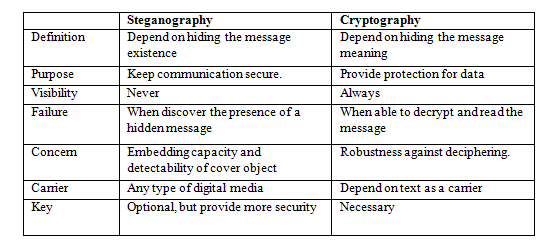
\includegraphics[width=35em, height=150mm]{figures/Pictures/Cypt vs Steg.png}}
\caption{Steganography vs Cryptography. Adapted from \cite{article2}}
\end{figure}

\chapter{Main Concepts}
Steganography is a method of hiding a hidden message within a cover image, audio file, or video file. The cover image acts as a vehicle for the hidden message, which is concealed within it via a steganography technique. To ensure safe communication, the algorithm defines how the secret message is encoded in the cover image, and a steganography key may also be employed. Understanding the fundamental fundamentals of steganography is essential for efficiently applying and employing this approach.

\vskip 3em
\begin{figure}[ht!]
\centering
\frame{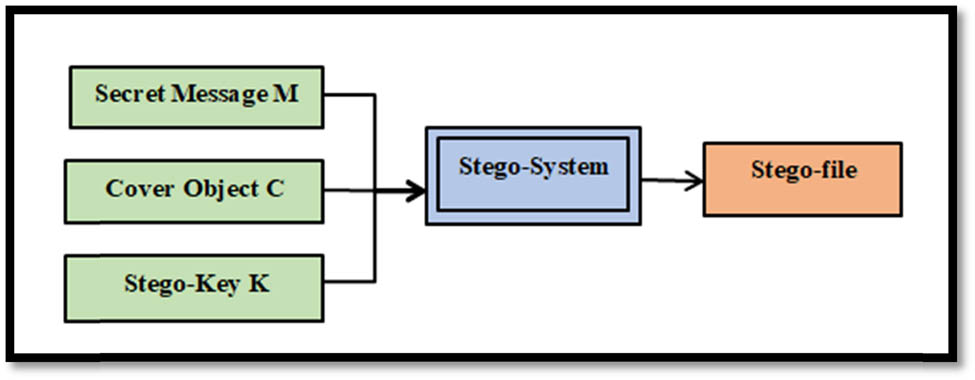
\includegraphics[width=35em, height=90mm]{figures/Pictures/Main Concepts.jpg}}
\caption{Steganography Main Concepts. Adapted from \cite{BaothmanEdhah+2021+903+919}}
\end{figure}


 \subsection{Cover Image}
 A cover image is the image in which the secret message is hidden. The cover image is chosen for its aesthetic complexity and resemblance to the original image. The cover image remains unmodified in image steganography, while the hidden message is embedded within it. The cover image can be in any format, including JPEG, PNG, and BMP.



\subsection{Secret Message}
 The cover image's secret message is the message we want to conceal. The hidden message can take any form, including text, audio, video, or images. The secret message's size is determined by the capacity of the cover image to store it. To ensure confidentiality and integrity, the secret message is encrypted using a cryptographic technique.


 \subsection{Steganography Algorithm}
 The steganography algorithm is used to incorporate the hidden message into the cover image. Least Significant Bit (LSB), Pixel Value Differencing (PVD), and Spread Spectrum Steganography are several steganography algorithms. The LSB algorithm substitutes the least significant bit of each pixel in the cover image with the secret message's corresponding bit. The PVD algorithm embeds the secret message in the cover image by comparing the difference between neighbouring pixels. By spreading the hidden message across various frequency channels, the Spread Spectrum Steganography method embeds it.

\begin{figure}[ht!]
\centering
\frame{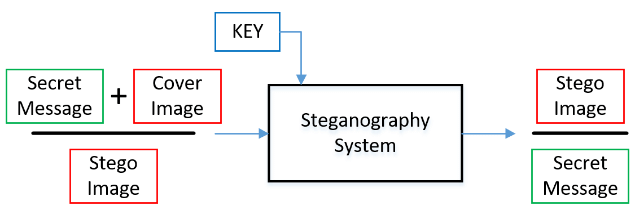
\includegraphics[width=35em, height=50mm]{figures/Pictures/LSB-based-image-steganography-system.png}}
\caption{LSB-based image steganography system. Adapted from \cite{article}}
\end{figure}


\begin{figure}[ht!]
\centering
     \frame{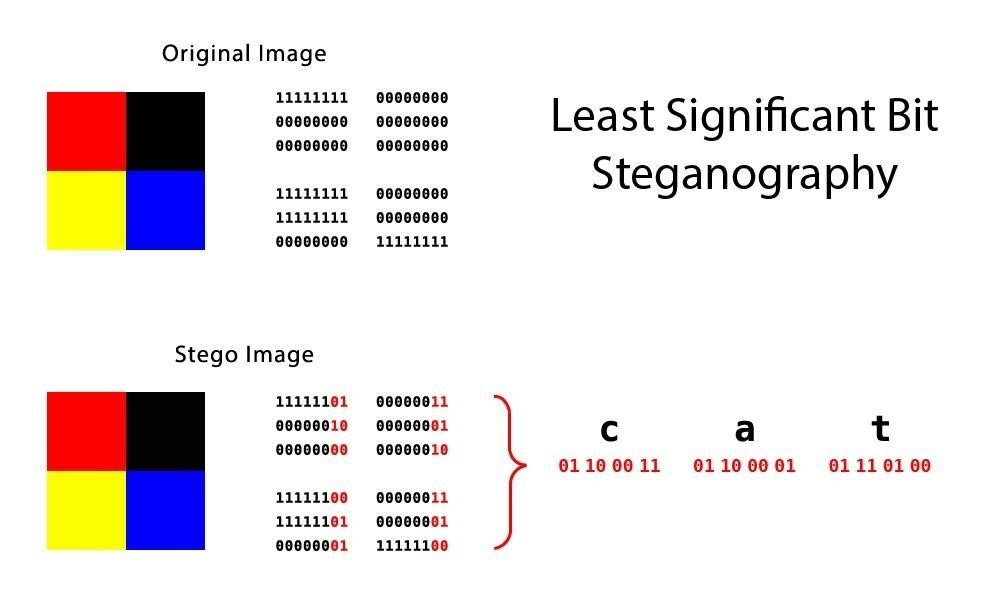
\includegraphics[width=35em, height=70mm]{figures/Pictures/LSB Steganography.jpg}}
     \caption{LSB Steganography \cite{link}}
\end{figure}


\begin{figure}[ht!]
\centering
\frame{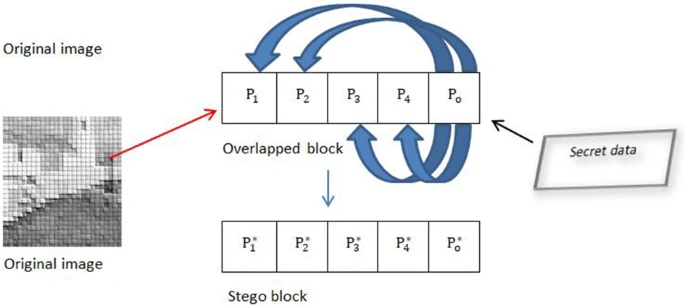
\includegraphics[width=35em, height=70mm]{figures/Pictures/Pixel Value Differencing(PVD) Image Steganography.png}}
\caption{Pixel Value Differencing Image Steganography. Adapted from \cite{article1}}
\end{figure}

 \subsection{Steganography Key}
A steganography key is a secret key that is used to encrypt the hidden message before it is included in the cover image. The steganography key is used to maintain the hidden message's confidentiality. Only the sender and intended recipient of the communication have access to the key. The hidden message is encrypted and decrypted using the steganography key. It is also used to choose which pixels in the cover image will contain the hidden message.

 \subsection{Key Takeaways}
 \vskip2em
In summary, the cover picture, secret message, steganography algorithm, and steganography key are the essential ideas of image steganography. These ideas are crucial for understanding how image steganography works and how to use it safely.
\vskip5em
\begin{figure}[ht!]
\centering
\frame{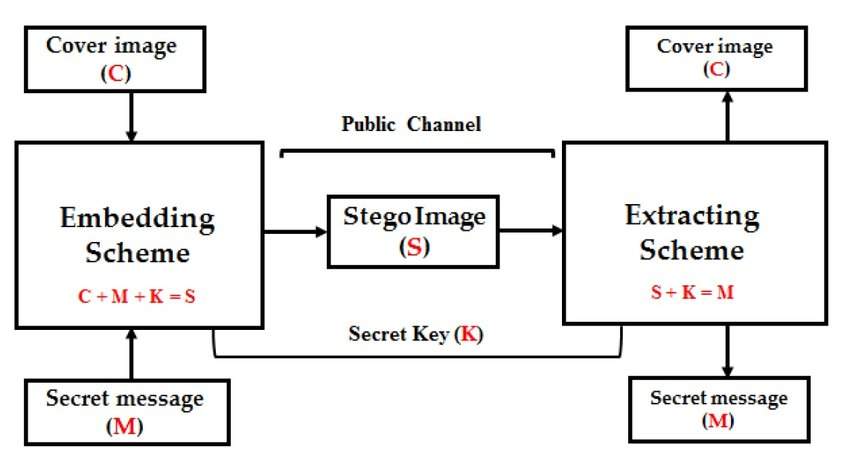
\includegraphics[width=35em, height=120mm]{figures/Pictures/The-basic-concept-of-the-steganography-arrangement-in-its-entirety.png}}
\caption{The basic concept of the steganography arrangement. Adapted from \cite{Hashim2021}.}
\end{figure}

\chapter{Main Components}

The four major components of steganography are embedding, extraction, cryptography, and user interface. The secret message is embedded, extracted, and encrypted using cryptography, and the user interface allows for system interaction. It is critical to grasp these crucial components in order to use steganography successfully and safely.
\vskip 3em
\begin{figure}[ht!]
\centering
     \frame{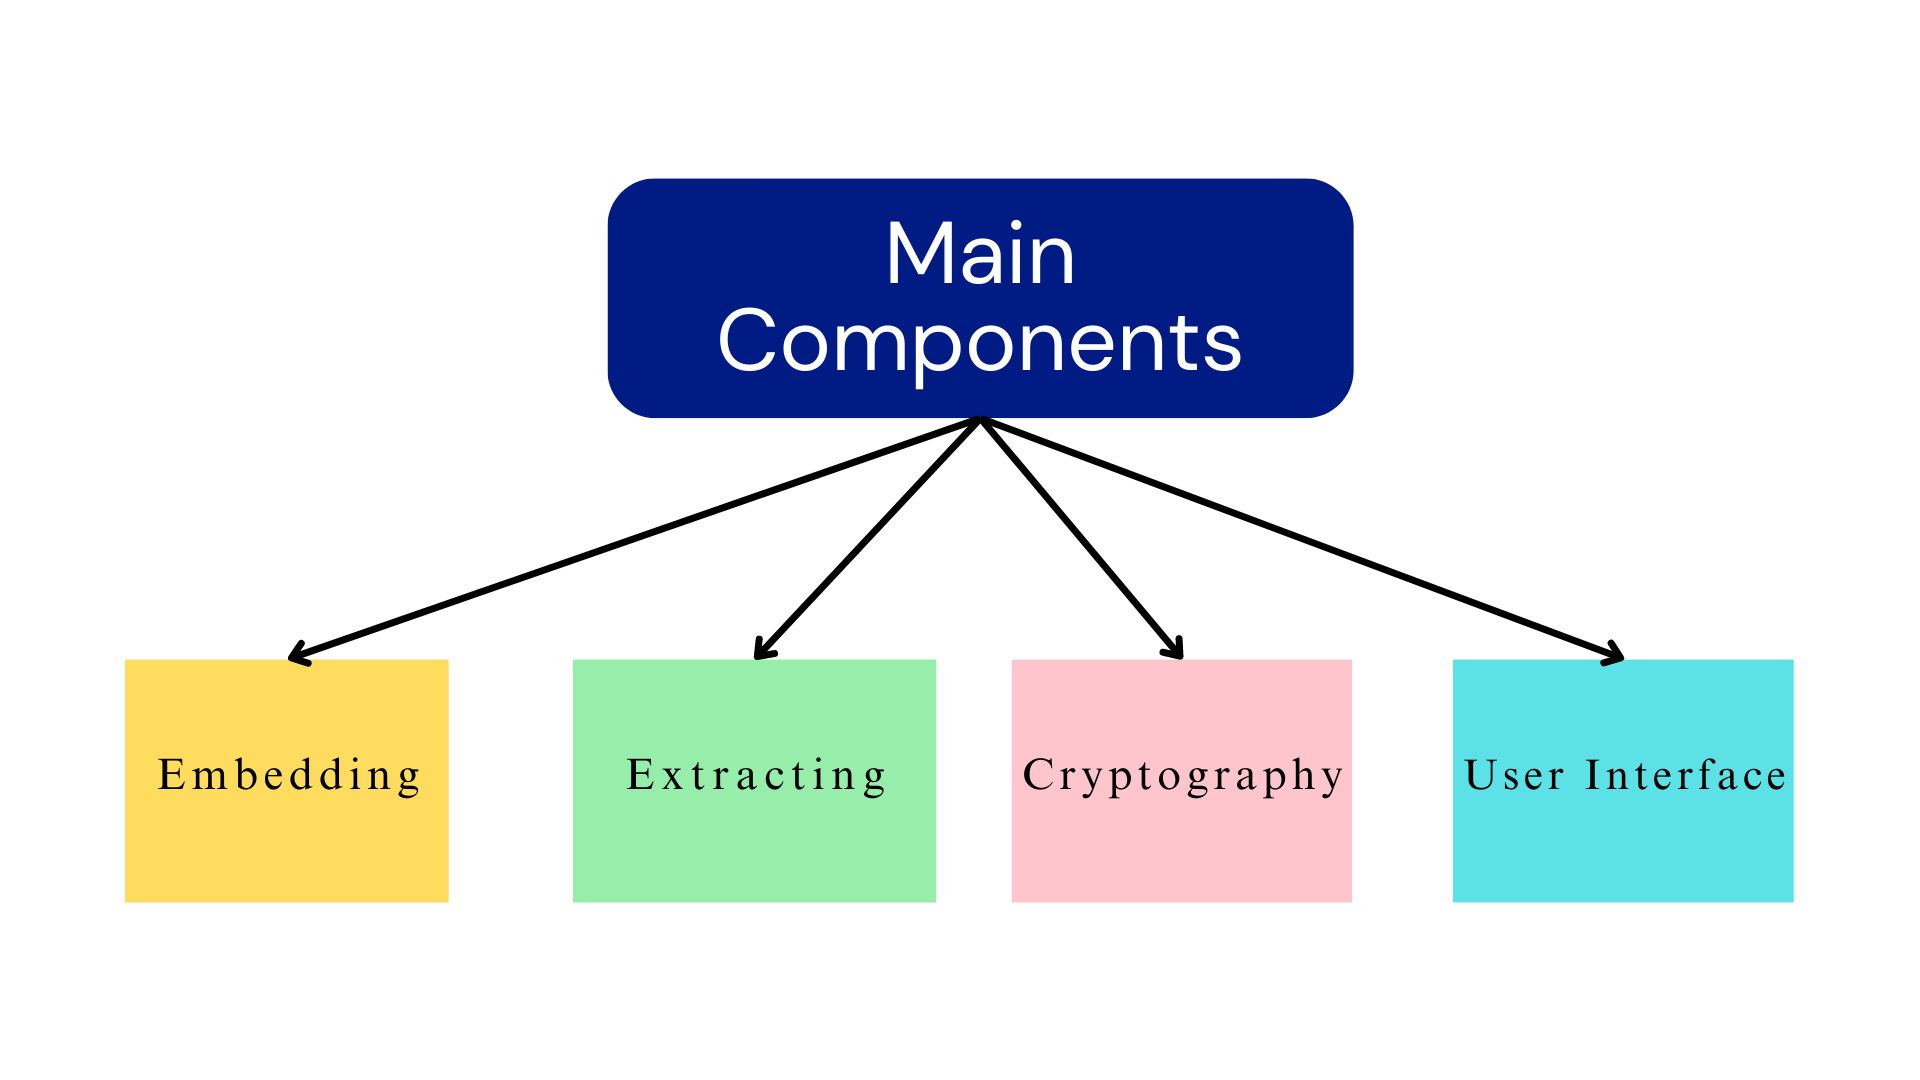
\includegraphics[width=35em, height=90mm]{figures/Pictures/Main Components.png}}
     \caption{Steganography Main Components}
\end{figure}

\subsection{Module for Embedding}
Using techniques like as LSB and PVD, the embedding module conceals the hidden message in the image file. The least significant bit of each pixel is replaced with a bit from the secret message using LSB, whereas PVD alters the difference between pixel values in consecutive pixels. PVD can embed the message more effectively but may distort the image, whereas LSB has little influence on image quality but is open to assaults.
\vskip1em
\textbf{The embedding module usually consists of the following steps:}

\begin{itemize}
\item Choose a carrier image and a hidden message.
\item Convert the encrypted message to binary format.
\item Disassemble the carrier image into individual pixels.
\item Using the embedding procedure, replace the bits of the carrier picture with the bits of the hidden message.
\item Save the changed image that contains the hidden message.
\end{itemize}
\subsection{Extraction Module}
The extraction module is in charge of obtaining the hidden message from the image file. The extraction procedure entails analyzing the image file and recovering the hidden message bits that were encoded in it. To retrieve the secret message, the extraction module employs the same procedures as the embedding module. To ensure that the extracted message is accurate and complete, the extraction module includes error correction methods.
\vskip2em
\textbf{The extraction module usually consists of the following steps:}

\begin{itemize}
\item Load the carrier picture with the hidden message.
\item Using the extraction algorithm, extract the bits of the secret message.
\item Convert the extracted bits back to the secret message format.
\item Using error correction methods, check the secret message's integrity.
\item Show the user the extracted secret message.
\end{itemize}
\vskip0.5em

\begin{figure}[ht!]
\centering
\frame{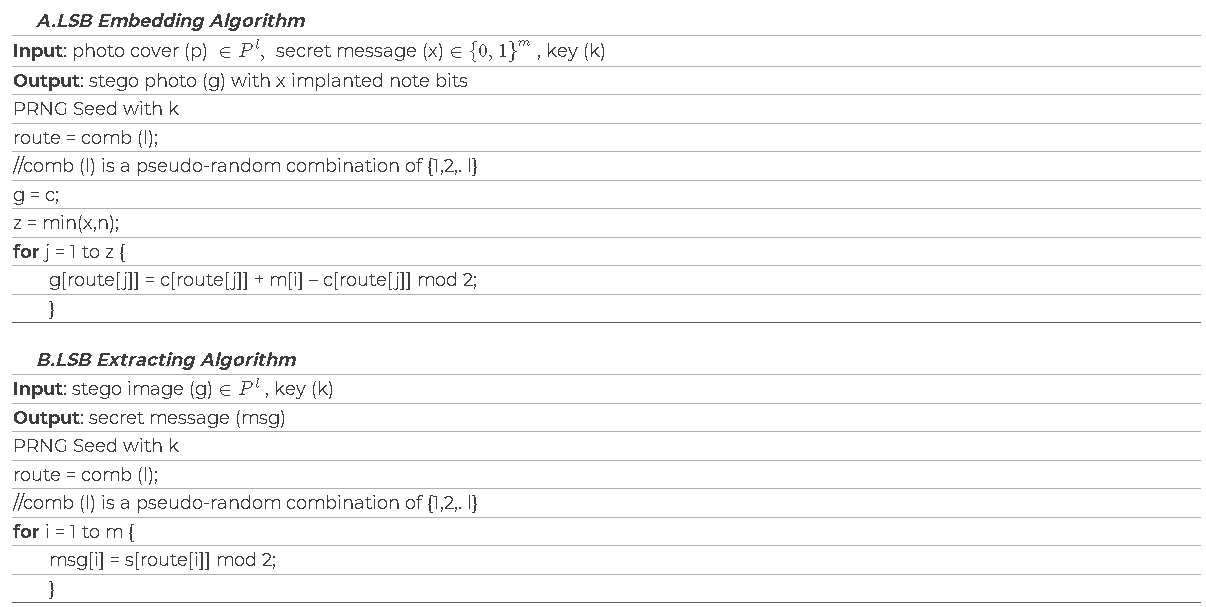
\includegraphics[width=37em, height=205mm]{figures/Pictures/LSB Embedding and Extracting Algorithms.png}}
\caption{LSB Embedding and Extracting Algorithms. Adapted from \cite{BaothmanEdhah+2021+903+919}}
\end{figure}

\subsection{Module of Cryptography}
The cryptography module is in charge of encrypting the secret message before embedding it in the picture file. The cryptography module ensures that the secret message is secure and that only the intended recipient has access to it. To encrypt the secret message, the cryptography module employs several encryption methods such as Advanced Encryption Standard (AES), Data Encryption Standard (DES), and Rivest-Shamir-Adleman (RSA).
\vskip0.5em

\textbf{Typically, the cryptography module includes the following steps:}

\begin{itemize}
\item Choose a secret message to encrypt.
\item Decide on a cryptography algorithm and create a key
\item Using the key and the cryptography technique, encrypt the secret message.
\item Using the embedding module, insert the encrypted message into the carrier image.
\item Distribute the key to the appropriate recipient
\end{itemize}

\subsection{User Interaction}
The user interface gives the steganography tool a graphical user interface (GUI). The user interface allows the user to select the carrier image and the secret message, as well as to configure the encryption technique and key and to start the embedding and extraction operations. The user interface is user-friendly and intuitive, allowing even non-technical individuals to utilize the steganography programme with ease.

\vskip0.5em

\textbf{User interface features:}

\begin{itemize}
\item An interface for picking the carrier image and the hidden message from files.
\item An encryption configuration interface that allows you to configure the encryption algorithm and key.
\item An embedding interface used to start the embedding process.
\item Using the embedding module, insert the encrypted message into the carrier image.
\item An extraction interface used to start the extraction process.
\item The retrieved secret message is shown using a message display interface.
\end{itemize}
 \subsection{Key Takeaways}
 \vskip1em
In summary, embedding, extraction, cryptography, and user interface are the four essential components of steganography. The embedding module hides the secret message within the carrier image, and the extraction module retrieves it. Before embedding the message, cryptography encrypts it, and the user interface allows users to engage with the steganography tool. Both the embedding and extraction modules require a number of processes, including error correction to ensure proper message retrieval. Overall, understanding these fundamental components is critical for using steganography efficiently and safely.
\vskip4em
 \begin{figure}[ht!]
\centering
     \frame{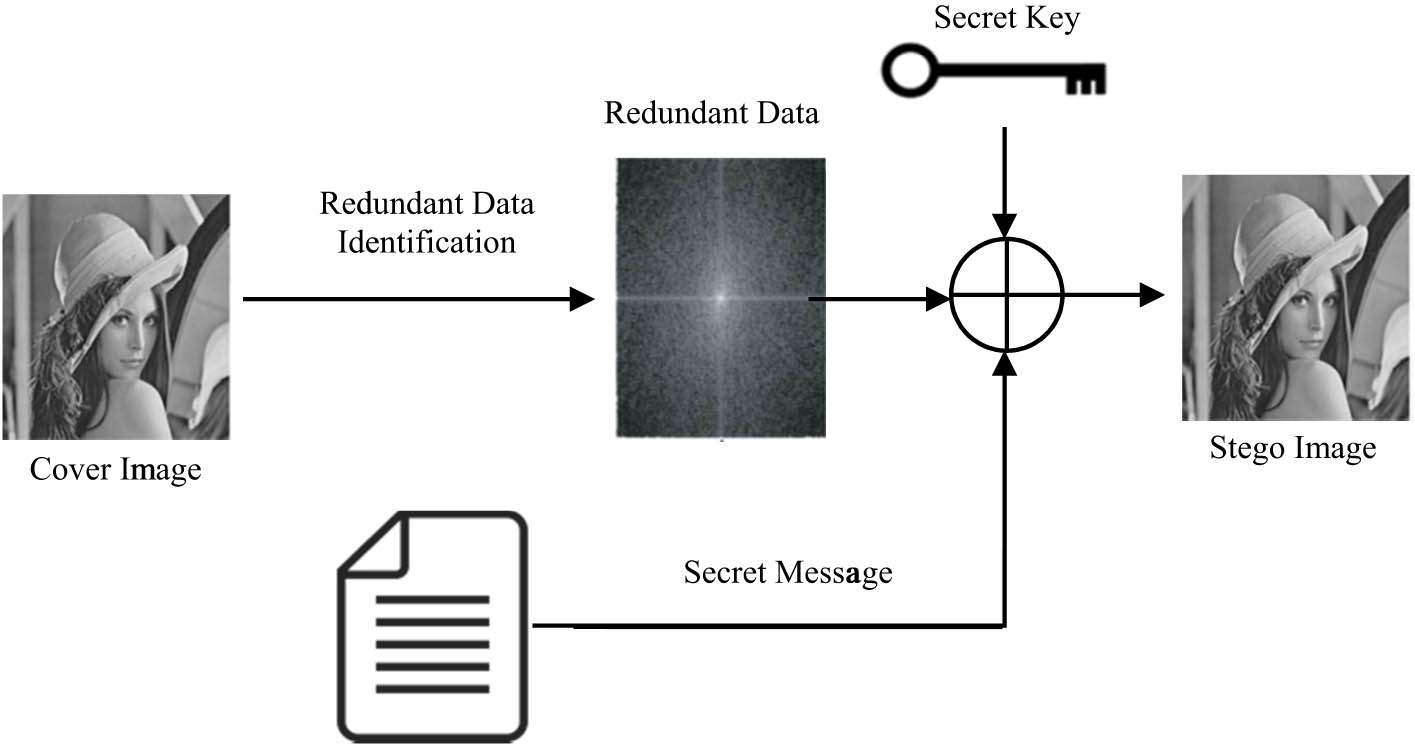
\includegraphics[width=35em, height=130mm]{figures/Pictures/Key Takeways Main Components.png}}
        \caption{LSB System. Adapted from \cite{BaothmanEdhah+2021+903+919}}
\end{figure}

\chapter{Functional Flow}
The step-by-step process of hiding a secret message behind a cover image to create a stego-image is referred to as steganography functional flow. Inputing the cover image and secret message, encrypting the secret message, embedding the encrypted message into the cover image, generating the stego-image, securely transmitting it, extracting the encrypted secret message, decrypting it, and displaying the hidden message are all common steps in this process. Understanding this functional flow is essential for using steganography for clandestine communication.


 \vskip 2em
\begin{figure}[ht!]
\centering
\frame{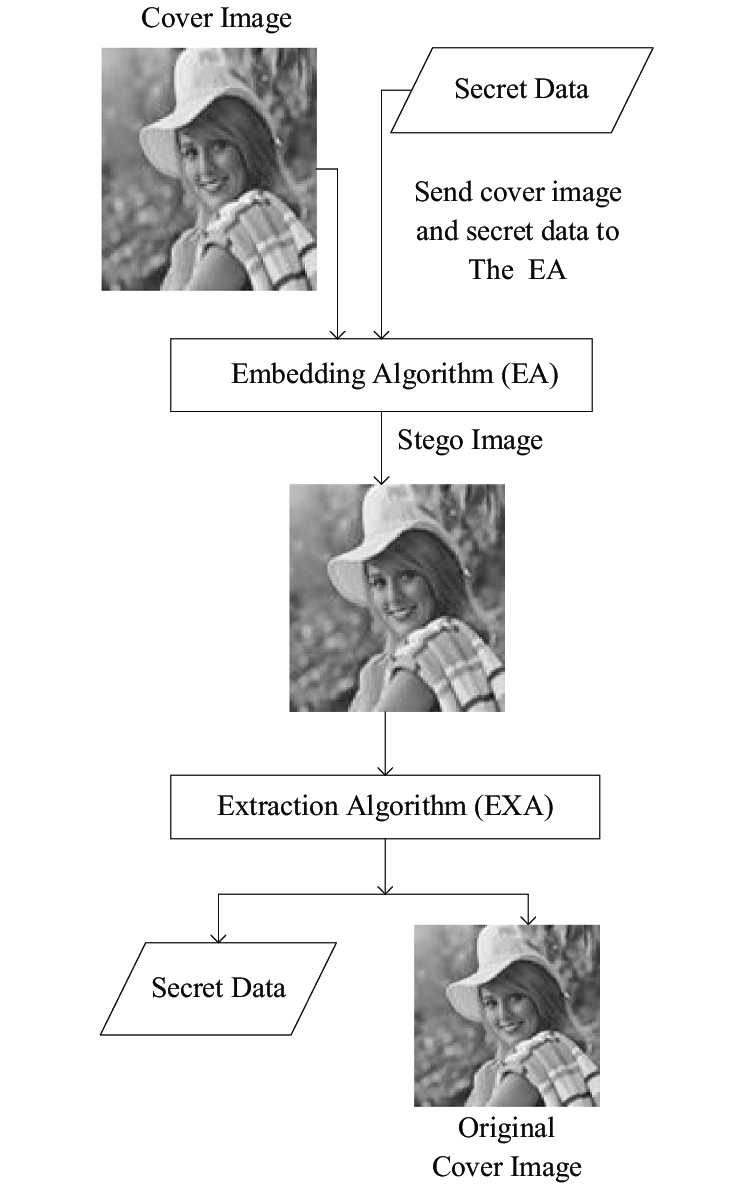
\includegraphics[width=35em, height=90mm]{figures/Pictures/Functional Flow.png}}
\caption{Steganography Functional Flow. Adapted from \cite{Maniriho2019}}
\end{figure}

\subsection{Input Cover Image and Secret Message}
The cover image and secret message are entered into the system by the user:
The user enters the input cover image and the secret message to be hidden in this phase. The cover picture can be any image that will be used as the carrier for the hidden message, such as a JPEG or PNG file. The secret message can be any data that needs to be kept private, such as text, audio, or video.
\vskip0.5em

\textbf{Here are some examples of cover images for an Image Steganography System:}

\begin{itemize}
\item Image of natural scenery, such as a landscape or a beach view.
\item Images of a creative nature, such as paintings or drawings.
\item Photos of commonplace objects, such as a cup, a book, or a pen.
\item Personal photographs, such as those of family members or pets.
\item Images that are abstract, such as colourful patterns or textures.
\end{itemize}
{\color{red}\textbf{The cover image for steganography should be carefully chosen to avoid suspicion. The chosen image should not raise any suspicions or appear suspicious. Following the submission of the cover image and secret message, the secret message is encrypted using a cryptographic technique to maintain confidentiality.}}

\subsection{Secret Message Encryption}
To guarantee confidentiality, the secret message provided by the user is encrypted in steganography. In the encryption process, a steganography key is utilised to generate a unique encryption pattern for each message. This key is a secret code known only to the sender and intended recipient, and it changes the arrangement of the message's bits, making deciphering difficult without it. Depending on the level of protection required and available processing power, many cryptographic methods can be used. Using a steganography algorithm, the encrypted message is subsequently inserted in the cover image.

\vskip3.8em

\subsection{Secret Message Embedding}
A steganography algorithm is used to embed the encrypted secret message into the cover image. The algorithm is intended to obscure the message in an unnoticeable manner. Depending on the security level and type of cover picture, various methods such as LSB, PVD, and SS can be employed. The steganography algorithm alters particular parts of the cover image to include the encrypted message while retaining the image's aesthetic look. A stego-picture including both the original cover image and the concealed message is created. It can be viewed and sent to the intended recipient.

\subsection{Generating the Stego-Image}
A stego-picture is created by merging the cover image and changed pixels carrying the encrypted secret message. The user is then shown the stego-image to confirm that it appears natural and does not raise suspicion. To avoid unauthorised access, the stego-image should be transferred using a secure connection. The user has the option of keeping the stego-image for personal use or sending it to the intended recipient.

\subsection{Transmitting the Stego-Image securely}
The stego-image can be communicated to the receiver using secure methods such as email or messaging apps, and encryption techniques such as TLS or SSL can be used to protect the data while it is being transmitted. Password security can also be used to ensure that the stego-image is only accessible to the intended recipient. If an unauthorised entity gains access, the steganography technique and key can be utilised to extract the secret message. The recipient can utilise the extraction module to obtain the message after it has been transmitted.

\subsection{Extracting the encrypted secret message}
The recipient uses the extraction module to extract the secret message from the stego-image, which is then decrypted using the same technique and key as the cryptography module. To avoid security issues, the extracted message is displayed to the receiver, who should keep it secure and erase the stego-image.

\subsection{Decrypting the encrypted secret message}
The steganography key is used by the extraction module to decipher the embedded secret message that was encrypted by the cryptography module. The encryption and decryption modules share the same algorithm and key. The extracted message is then shown to the intended recipient, who must maintain the key secret in order for the message to be extracted from the stego-image. For the intended recipient to extract and read the buried secret message, the seventh step is critical.

\subsection{Displaying the secret message}
The original message is displayed to the receiver when the extraction module decrypts the secret message using the steganography key. The recipient can then take appropriate actions based on its contents. Because the decrypted message may contain critical information, it must be kept discreet and safe. The completion of the final step indicates that the secret message was securely transferred to the recipient and was not intercepted. The eighth and last phase of an Image Steganography System is critical for the recipient to access and interpret the secret message and take necessary actions as a result of it.

\subsection{Key Takeaways}
To summarise, the functional flow of steganography entails hiding a hidden message beneath a cover image to form a stego-image. To guarantee confidentiality, the input cover image and secret message are encrypted, and a steganography algorithm is employed to embed the encrypted message into the cover image in an imperceptible manner. Using encryption techniques and password security, the stego-image can be securely transferred to the intended recipient, and the receiver can extract and decrypt the concealed message using the steganography key. The original communication is shown to the receiver, who must keep it private and secure. Understanding the functional flow of steganography is critical for employing it for covert communication.

\chapter{Main existing solutions}

\section{ SSIS (Spread Spectrum Image Steganography) }
Spread Spectrum Image Steganography (SSIS) works by storing a message as Gaussian noise in an image (Marvel, Boncelet, and Retter 1998, Marvel et al. 1999). At low noise power levels, the image degradation is undetectable by the human eye, while at higher levels. the noise appears as speckles or “snow.” The procedure is broken down into the following key steps, which are shown in figure :
\vskip2em
\begin{itemize}
\item Create encoded message by adding redundancy via error-correcting code.
\item Add padding to make the encoded message the same size as the image.
\item Interleave the encoded message.
\item Generate a pseudorandom noise sequence, n.
\item  Use encoded message, m, to modulate the the sequence, generating noise, s.
\item Combine the noise with the original image, f. 
\end{itemize}
\vskip8em
\subsection{Main Characteristics}
\begin{itemize}
\item SSIS is a type of steganography that involves embedding secret data within an image without altering the perceptual quality of the image.
\item It is based on the spread spectrum communication technique, which involves spreading the secret data signal over a wide bandwidth.
\item Interleave the encoded message.
\item The spread spectrum technique used in SSIS helps to make the embedded data more resistant to detection and removal by attackers.
\item SSIS is a reversible process, meaning that the secret message can be extracted from the image without any loss of information.
\end{itemize}
\vskip3em
\begin{figure}[ht!]
\centering
\frame{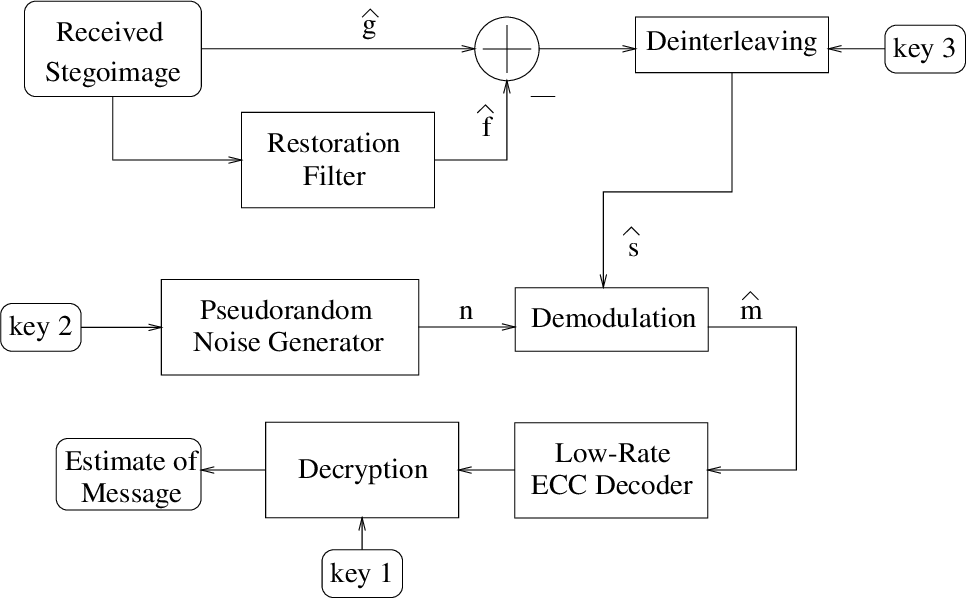
\includegraphics[width=35em, height=100mm]{figures/Pictures/SSID.png}}
\caption{Spread spectrum image steganography. Adapted from \cite{Marvel1999SpreadSI}}
\label{fig:ssid}
\end{figure}
\subsection{Advantages}
\begin{itemize}
\item SSIS is a robust technique for hiding secret data within an image, making it more difficult for attackers to detect and remove the embedded data.
\item SSIS can be used for a wide range of applications, such as in digital watermarking, copyright protection, and covert communication.
\item The use of spread spectrum communication helps to make the embedded data more resistant to attacks such as noise addition and cropping
\end{itemize}

\subsection{Limitations}
\begin{itemize}
\item SSIS requires a large bandwidth to spread the secret data signal, which can be a limitation in situations where bandwidth is limited or expensive.
\item The use of SSIS can result in a slight degradation of the image quality, although this can be minimized through careful selection of the embedding parameters.
\item SSIS can be vulnerable to attacks such as correlation and statistical analysis, which can be used to detect the presence of the embedded data.
\end{itemize}

\subsection{Conclusion}
{\color{black}\textbf{In conclusion, SSIS is an effective and adaptable method for embedding hidden messages in images via spread spectrum communication. It has a large number of uses in digital watermarking, copyright protection, and clandestine communication, as well as high capacity data concealment, resistance to attacks such cropping and rotation. To prevent picture degradation, SSIS must be used with care as it is susceptible to statistical attacks. SSIS is a useful instrument for safe communication and data protection in the modern world.}}

\vskip6em

\section{BATCH steganography}
Batch steganography is a technique for hiding a secret message within multiple files simultaneously, such as images, videos, or documents. The process involves dividing the secret message into small pieces and embedding each piece in a different file using a steganographic algorithm. The files containing the embedded message can be distributed publicly, and only the intended recipient who knows the extraction process can retrieve the original message.
\vskip2em
\begin{figure}[ht!]
\centering
\frame{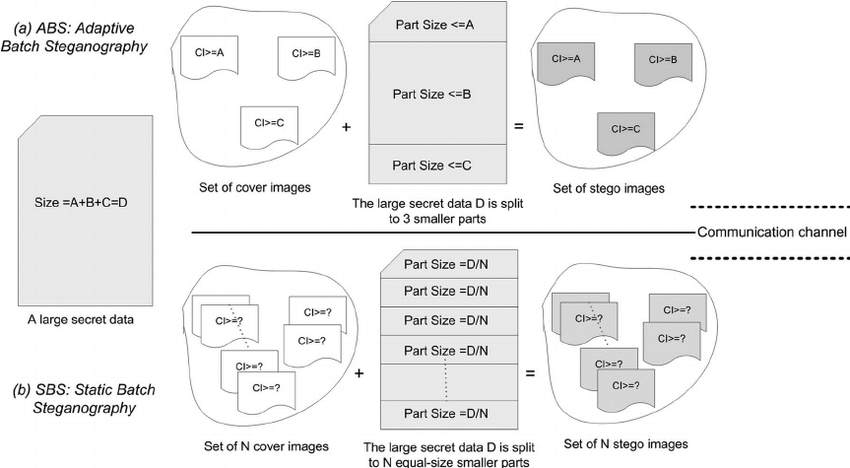
\includegraphics[width=35em, height=85mm]{figures/Pictures/Batch-steganography-a-adaptive-batch-steganography-and-b-static-batch.png}}
\caption{Batch image steganography. Adapted from \cite{batch}}
\label{fig:ssid}
\end{figure}

\subsection{Main Characteristics}
\begin{itemize}
\item Batch steganography involves embedding a secret message within multiple files, such as images or documents, to increase the overall capacity of the message.
\item Batch steganography can be used to hide a secret message in a variety of file formats, making it more difficult for attackers to detect the presence of the message.
\item Batch steganography can be used to embed the secret message in a specific order, which can be used to convey additional information.
\end{itemize}

\subsection{Advantages}
\begin{itemize}
\item Batch steganography allows for high-capacity data hiding, as the secret message can be divided among multiple files.
\item Batch steganography can be used to increase the robustness of the hidden message, as attackers would need to detect and extract the message from multiple files rather than a single file.
\item Batch steganography can be used to hide the existence of the secret message, as it can be difficult for attackers to identify the specific files that contain the message.
\end{itemize}

\subsection{Limitations}
\begin{itemize}
\item Batch steganography can be time-consuming and resource-intensive, as it requires the embedding of the secret message in multiple files.
\item The use of batch steganography can result in a loss of data fidelity or perceptual quality in the files containing the hidden message.
\item The use of batch steganography may be detectable through statistical analysis, as the distribution of the data in the files may be altered by the embedding process.
\end{itemize}
\vskip3em
\subsection{Conclusion}
\textbf{In summary, batch steganography is a powerful technique for hiding secret messages in multiple files simultaneously, providing high-capacity data hiding and increased robustness. However, the use of batch steganography can be time-consuming and resource-intensive, and it may result in a loss of data fidelity or detectability through statistical analysis.}
\vskip4.9em
\section{PIT (Pixel Indicator Technique)}
The Pixel Indicator Technique is a steganography technique used to conceal secret information in the least significant bit of a pixel indicator, which is a flag that indicates whether a pixel has been updated. The hidden message is encoded in the least significant bit (LSB) of specific image pixels. These pixels are chosen based on their RGB values, and the message is embedded by changing the value of the least significant bit.
\vskip2em

\underline{\color{red}\textbf{How it works:}}
\begin{itemize}
\item The cover image is separated into non-overlapping pixel blocks.
\item The most significant bit (MSB) of each pixel in each block is altered to encode a secret message.
\item Each pixel in the block's least significant bit (LSB) is updated to indicate whether or not it includes concealed information.
\end{itemize}
\vskip2em
\underline{\color{red}\textbf{Diagram:}}
\vskip2em
\begin{figure}[ht!]
\centering
\frame{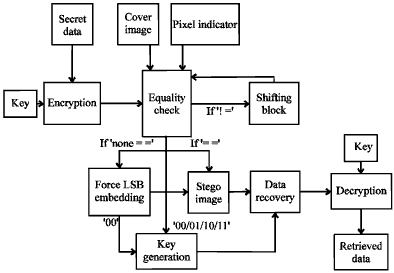
\includegraphics[width=35em, height=75mm]{figures/Pictures/PIT Diagram.png}}
\caption{Block Diagram for PIT. Adapted from \cite{ref}}
\end{figure}

\vskip1em.

\underline{\color{red}\textbf{Hiding Process:}}
\begin{figure}[ht!]
\centering
\frame{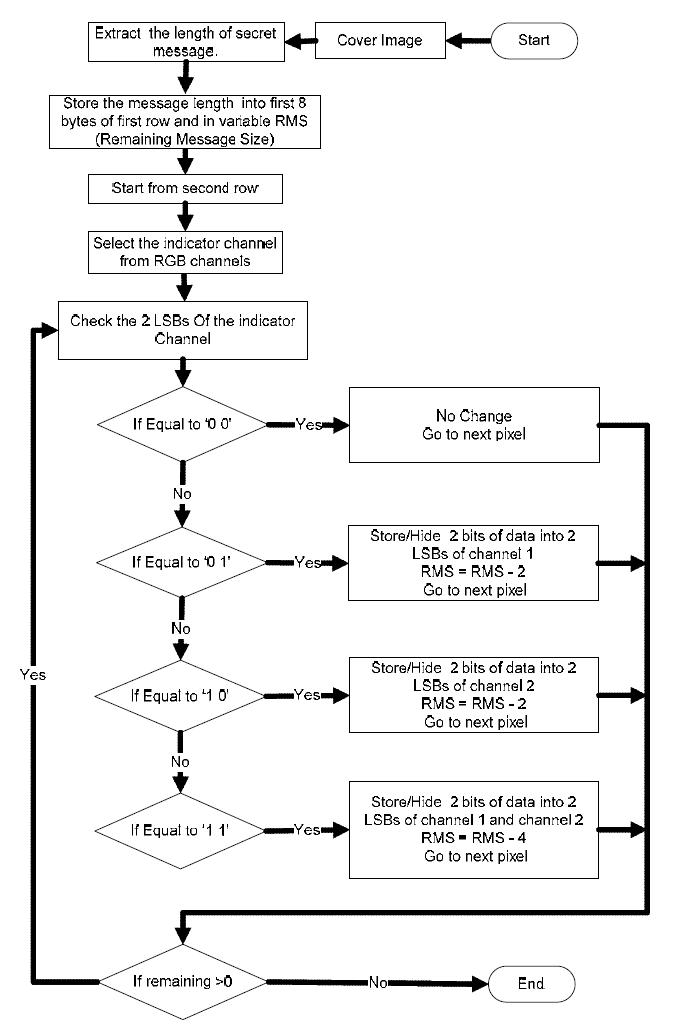
\includegraphics[width=35em, height=98mm]{figures/Pictures/PIT Hiding Process.png}}
\caption{PIT Hiding Process. Adapted from \cite{Gutub2010PixelIT}}
\end{figure}

\underline{\color{red}\textbf{Extraction Process:}}
\begin{figure}[ht!]
\centering
\frame{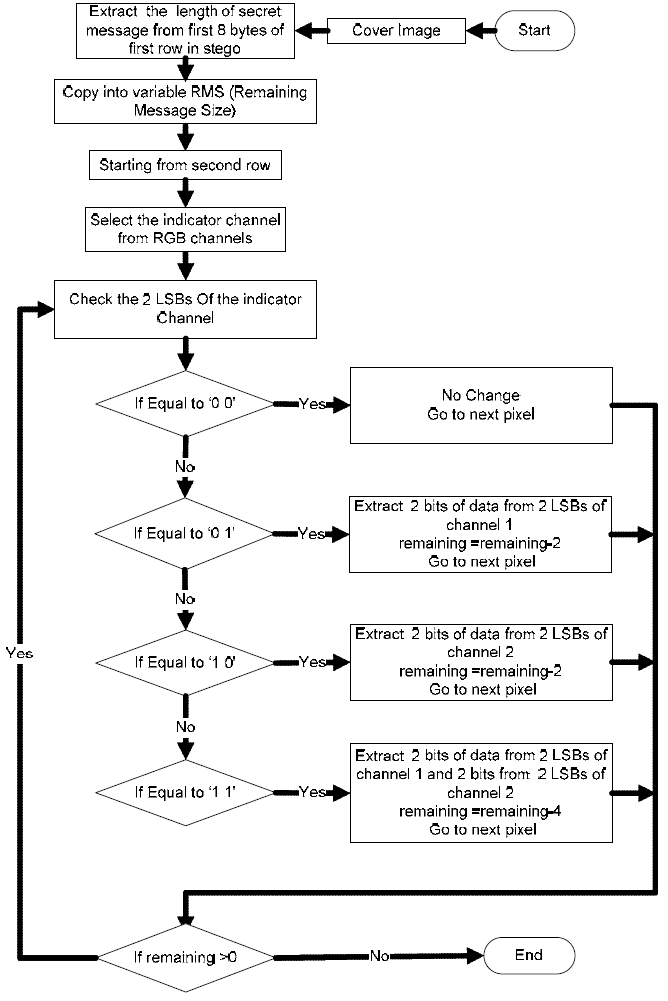
\includegraphics[width=35em, height=97mm]{figures/Pictures/PIT Extraction Process.png}}
\caption{PIT Extractions Process. Adapted from \cite{Gutub2010PixelIT}}
\end{figure}


\subsection{Main Characteristics}
\begin{itemize}
\item The embedding procedure is simple and quick. 
\item The resulting stego-image resembles the original image in appearance.
\item The method is resistant to attacks that change the image on a global scale.
\item Without the original cover image, the message can be extracted.
\end{itemize}

\subsection{Advantages}
\begin{itemize}
\item High capacity for message embedding
\item The cover image has minimal distortion. from multiple files rather than a single file.
\item Simple to implement and use
\item Effective against global image attacks
\end{itemize}

\subsection{Limitations}
\begin{itemize}
\item Vulnerable to attacks that specifically target the pixels used for embedding
\item Not appropriate for highly compressed images
\item If too many pixels are modified, image quality may suffer.
\end{itemize}
\vskip3em
\subsection{Conclusion}
\textbf{Despite its limitations, the Pixel Indicator Technique remains a popular and effective method of steganography due to its ease of use, high capacity, and resistance to attacks. It is important to note, however, that the success of this technique is heavily dependent on the indicator matrix chosen, and it may not be appropriate for all types of cover images.}

\section{BPCS (Bit-Plane Complexity Segmentation)}
The Bit-Plane Complexity Segmentation is a type of steganography in which a secret message is embedded in an image's complex bit planes. The complex bit planes are chosen for their randomness and complexity, making detection of the embedded message difficult.
\vskip2em

\underline{\color{red}\textbf{How it works:}}
\begin{itemize}
\item Select the cover image and secret message
\item Analyze the image and select the complex bit planes
\item Embed the secret message into the complex bit planes using a specific algorithm.
\item Send the stego-image to the receiver
\item Extract the secret message by reversing the embedding algorithm
\end{itemize}
\vskip1em

\underline{\color{red}\textbf{Hiding and Extracting Data:}}
The BPCS approach conceals data by partitioning the image into non-overlapping blocks and embedding bits in each block's most complicated bit-planes.
The receiver must first identify the complex bit-planes and block locations in order to retrieve the secret data.
\vskip1em
\begin{figure}[ht!]
\centering
\frame{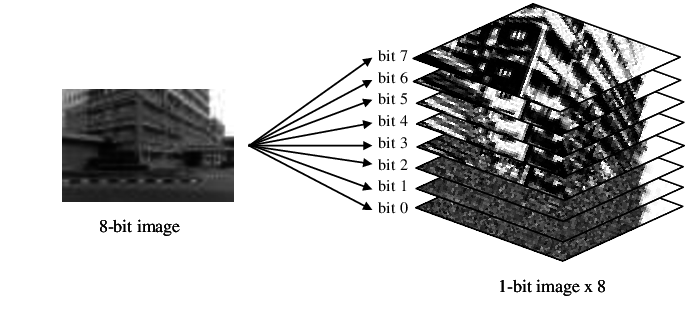
\includegraphics[width=35em, height=80mm]{figures/Pictures/8-bit image decomposed into 8 binary images prior to the embedding process..png}}
\caption{8-bit image is decomposed into 8 binary images prior to the embedding process.\cite{KHAIRE}}
\end{figure}


\subsection{Main Characteristics}
\begin{itemize}
\item The embedding procedure necessitates a significant amount of processing power.
\item The approach is immune to attacks that change the image on a global scale.
\item Without the original cover art, the message can be extracted.
\item Without understanding of the embedding algorithm, detecting the approach is challenging.
\end{itemize}

\subsection{Advantages}
\begin{itemize}
\item High capacity for message embedding.
\item The approach is immune to attacks that change the image on a global scale.
\item Without understanding of the algorithm, detecting the message is challenging.
\item Suitable for photos that have been heavily compressed.
\end{itemize}

\subsection{Limitations}
\begin{itemize}
\item The embedding procedure is time-consuming and computationally demanding.
\item The procedure may cause distortion to the cover image.
\item Attacks that target the precise bit planes utilised for embedding are possible.
\item The process is more difficult to implement and employ than other steganography techniques.
\end{itemize}

\subsection{Conclusion}
\textbf{In conclusion, the Bit-Plane Complexity Segmentation technique has been demonstrated to be a reliable and secure steganography method with high capacity and resistance to attacks. However, the requirement for large cover images and longer embedding times may limit its use. It is also worth noting that the technique's success is dependent on the right selection of threshold values, which can affect the visual quality of the stego image.}

\section{LSB (Least Significant Bit)}
In LSB (Least Significant Bit) steganography, the secret message bit is substituted for the least significant bit of each pixel value in the cover image. It is a preferred option for hiding hidden messages since the changes are frequently modest and hard to notice visually.
\vskip2em

\underline{\color{red}\textbf{How it works:}}
\begin{itemize}
\item Retrieve the binary representation of the secret message.
\item Begin with the first pixel in the upper-left corner of the cover image.
\item For each bit of the secret message, replace the least significant bit of the current pixel with the bit of the secret message.
\item Move to the next pixel in the cover image and repeat step 3 until all the bits of the secret message have been embedded.
\item If the end of the cover image is reached before all the bits of the secret message have been embedded, wrap around to the beginning of the cover image and continue embedding the remaining bits.
\item The resulting image can be transmitted or stored with the hidden message embedded within it. To extract the message, the same process is used to retrieve the least significant bits of the pixels and convert them back to the original message bits.
\end{itemize}
\vskip1em

\underline{\color{red}\textbf{Diagram:}}
\begin{figure}[ht!]
\centering
\frame{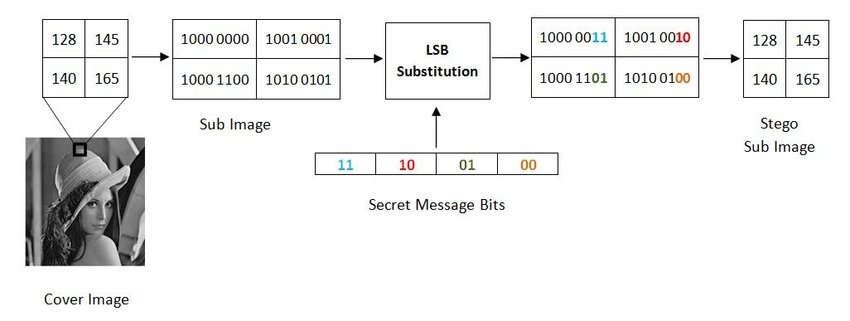
\includegraphics[width=35em, height=50mm]{figures/Pictures/Digram of LSB substitution techniques.png}}
\caption{Digram of LSB substitution techniques.\cite{LSB}}
\end{figure}

\underline{\color{red}\textbf{Hiding Process:}}
\begin{itemize}
\item Put the cover photo and the hidden message in binary format.
\item Determine the number of LSBs that can be changed per RGB color channel without affecting the cover picture, which is usually 1-2 bits.
\item Divide the secret message into equal-sized pieces corresponding to the number of LSBs in the cover picture.
\item Change the LSBs of the cover picture for each message piece to match the binary values of that piece.
\item Save the updated picture as the stego-image.
\end{itemize}
\vskip1em

\underline{\color{red}\textbf{Extraction Process:}}
\begin{itemize}
\item Put the stego-image on.
\item Find the quantity of least significant bits (LSBs) needed to encrypt the secret message.
\item The binary values of the concealed message chunks may be obtained by separating the LSBs from each pixel in the stego-image.
\item The secret message may be obtained by combining the binary parts.
\end{itemize}
\vskip1em

\begin{figure}[ht!]
\centering
\frame{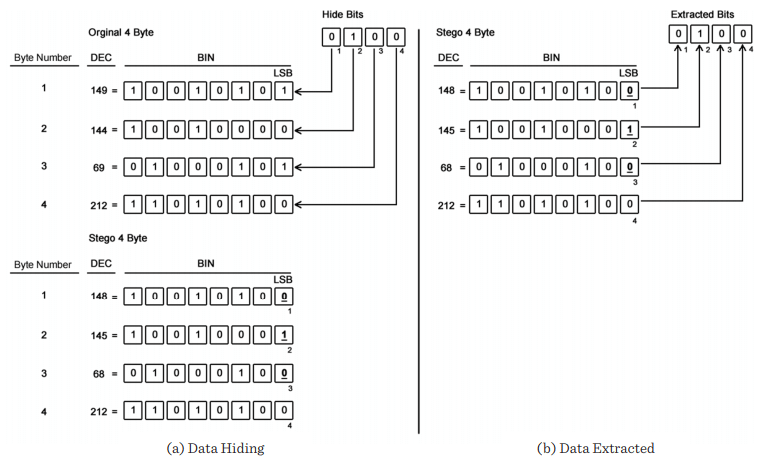
\includegraphics[width=35em, height=60mm]{figures/Pictures/Hiding-and-extracting-data-with-LSB-method-a-Hiding-data-b-Extracting-data.png}}
\caption{Hiding and extracting data with LSB. Adapted From \cite{Hidings}}
\end{figure}

\subsection{Main Characteristics}
\begin{itemize}
\item A straightforward and effective steganography method is LSB.
\item It may be used with a variety of cover material, including as pictures, audio, and video.
\item The changes to the cover picture are often subtle and undetectable to the naked eye.
\end{itemize}

\subsection{Advantages}
\begin{itemize}
\item Implementing LSB steganography is simple and doesn't require a lot of computer power.
\item Without noticeably lowering the image's quality, it may conceal a lot of info in cover photos.
\item Many software tools and libraries support and use LSB steganography.
\end{itemize}

\subsection{Limitations}
\begin{itemize}
\item Attacks that look for concealed messages via statistical analysis can find them using LSB steganography.
\item It is also susceptible to attacks that change the cover image's LSBs, which might lead to the concealed message being lost or being shown to unauthorized people.
\item Because LSB steganography is not very reliable, even minor changes to the cover image can result in the hidden message being lost or altered.
\end{itemize}

\subsection{Conclusion}
\textbf{Finally, LSB steganography is a frequently used and simple technique for concealing data within digital photographs. It has various advantages, including high embedding capacity and message imperceptibility. However, it has several limitations, including vulnerability to attacks, image quality degradation, and the inability to embed large messages.}

\section{PVD (Pixel-Value Differencing)}
The hidden message is concealed using the PVD (Pixel-Value Differencing) steganography method by using the difference between adjacent pixel values in the cover picture. Compared to LSB steganography, PVD steganography is more durable and more resistant to statistical analysis-based assaults.
\vskip2em

\underline{\color{red}\textbf{How it works:}}
\begin{enumerate}
\item Calculate the difference between adjacent pixel values in the cover picture.
\item Alter the difference value between two successive pixels to insert the hidden message.
\item Ensure that the modifications are minor, and the difference values stay within a predetermined range.
\end{enumerate}
\vskip2em

\underline{\color{red}\textbf{Diagram:}}
\vskip2em
\begin{figure}[ht!]
\centering
\frame{\includegraphics[width=30em, height=100mm]{figures/Pictures/PVD diagram of a 3 × 3-pixel block..jpg}}
\caption{PVD diagram of a 3 × 3-pixel block. Adapted From\cite{pvd}}
\end{figure}

\underline{\color{red}\textbf{Hiding Process:}}
\begin{itemize}
\item Create a binary bit stream from the secret message.
\item Create non-overlapping blocks of size m x n.
\item Compute the edge maps for each block using an edge detection operator.
\item Change the LSB of a pixel with a strong edge to the corresponding bit of the binary stream for each block.
\item Repeat step 4 for each bit in the binary stream.
\item Combine all the changed blocks to create the stego-image.
\end{itemize}
\vskip1em

\begin{figure}[ht!]
\centering
\frame{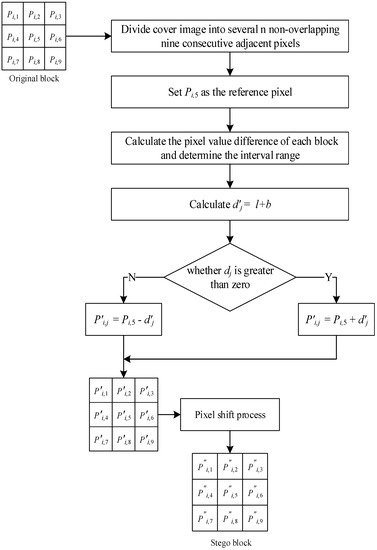
\includegraphics[width=35em, height=140mm]{figures/Pictures/PVD embedding procedure..jpg}}
\caption{PVD embedding procedure. Adapted From \cite{pvd}}
\end{figure}

\underline{\color{red}\textbf{Extraction Process:}}
\begin{itemize}
\item Create non-overlapping blocks of size m x n from the stego-image.
\item Compute the edge maps for each block using an appropriate edge detection operator.
\item Calculate the difference between the original and stego versions of each block.
\item Concatenate the LSBs of the difference values from step 3 to reveal the hidden message.
\end{itemize}
\vskip1em

\begin{figure}[ht!]
\centering
\frame{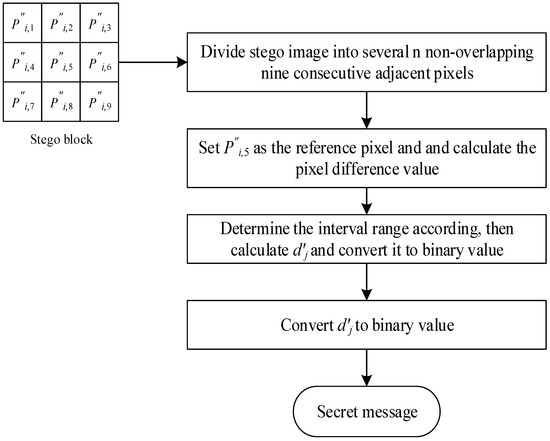
\includegraphics[width=35em, height=100mm]{figures/Pictures/PVD extracting procedure.jpg}}
\caption{PVD extracting procedure. Adapted From \cite{pvd}}
\end{figure}

\subsection{Main Characteristics}
\begin{itemize}
\item A straightforward and effective steganography method is LSB.
\item It may be used with a variety of cover material, including as pictures, audio, and video.
\item The changes to the cover picture are often subtle and undetectable to the naked eye.
\end{itemize}

\subsection{Advantages}
\begin{itemize}
\item Implementing LSB steganography is simple and doesn't require a lot of computer power.
\item Without noticeably lowering the image's quality, it may conceal a lot of info in cover photos.
\item Many software tools and libraries support and use LSB steganography.
\end{itemize}

\subsection{Limitations}
\begin{itemize}
\item Attacks that look for concealed messages via statistical analysis can find them using LSB steganography.
\item It is also susceptible to attacks that change the cover image's LSBs, which might lead to the concealed message being lost or being shown to unauthorized people.
\item Because LSB steganography is not very reliable, even minor changes to the cover image can result in the hidden message being lost or altered.
\end{itemize}
\vskip3em
\subsection{Conclusion}
\textbf{Finally, PVD steganography is a more advanced technique that seeks to overcome the limitations of LSB. It improves security, imperceptibility, and resistance to attacks. It does, however, have limits, such as a reduced embedding capacity and the complexity of the encoding and decoding operations.
.}

\chapter{Critique of  existing solutions}

\section{ SSIS Criticism }
Attacks that take advantage of well-known weaknesses in the encryption technique may leave SSIS open to risk. For instance, to decrypt the concealed message, an attacker might be able to estimate the encryption key or take advantage of algorithmic weaknesses. To guarantee that SSIS is utilized properly and that the intended level of security is attained, careful evaluation of these restrictions is required. Overall, SSIS can be a useful steganography technique, but it's important to weigh its advantages and disadvantages when deciding which steganography method is best for a given application.
\section{ BATCH steganography Criticism }
With the ability to embed and extract messages from many files, batch steganography can be more difficult to build and utilize than single-file steganography systems. To use batch steganography effectively and achieve the needed level of security, several restrictions must be carefully taken into account. Overall, batch steganography can be a useful steganography technique, but it's crucial to weigh its advantages and disadvantages when deciding which steganography method is best for a given application.
\section{ PIT Criticism }
While PIT has some benefits, such as being easy to implement and not requiring the original image for extraction, it also has some significant drawbacks. PIT is vulnerable to statistical analysis attacks, in which an attacker can detect hidden information by analysing statistical features of the cover image. Furthermore, PIT has a limited embedding capacity, which means it can only hide a limited amount of information in a single image.

\section{ BPCS Steganography Criticism }
While BPCS Steganography has some advantages, such as high security and embedding capacity, it also has some significant drawbacks. One of the main drawbacks of BPCS is that it requires a larger cover image than other steganography techniques, making it unsuitable for some applications. Furthermore, the embedding process can be computationally demanding, which can be difficult when working with large images or datasets. Finally, BPCS is vulnerable to some attacks, such as the RS analysis attack, which can reveal the presence of hidden data in the cover image by analysing the relationship between bit planes.

\section{ LSB Criticism }
Because of its simplicity, the LSB approach is commonly employed, although it has a limited capability for hiding data in high-resolution photographs and might create visual distortion to the cover image, making concealed information simpler to discover. It's also susceptible to compression, which can lead to the loss or corruption of buried data.

\section{ PVD Criticism }
PVD has advantages such as increased data hiding capacity and less aesthetic distortion to the cover image, as well as being compression resistant. It does, however, have drawbacks such as high computer resource requirements and sensitivity to noise and signal changes. Furthermore, due to specific requirements for colour space and image size, the PVD method may not be appropriate for some types of cover images or applications.

\chapter{SSIS UML Design}
\section{Use case diagram}
\begin{figure}[ht!]
\centering
\frame{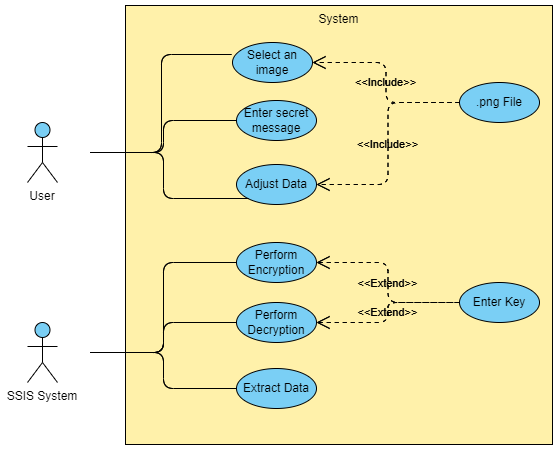
\includegraphics[width=35em, height=137mm]{figures/UML Design/Use Case Diagram.png}}
\caption{SSIS Use Case Diagram.}
\end{figure}
\section{Sequence diagram}
\vskip2em
\begin{figure}[ht!]
\centering
\frame{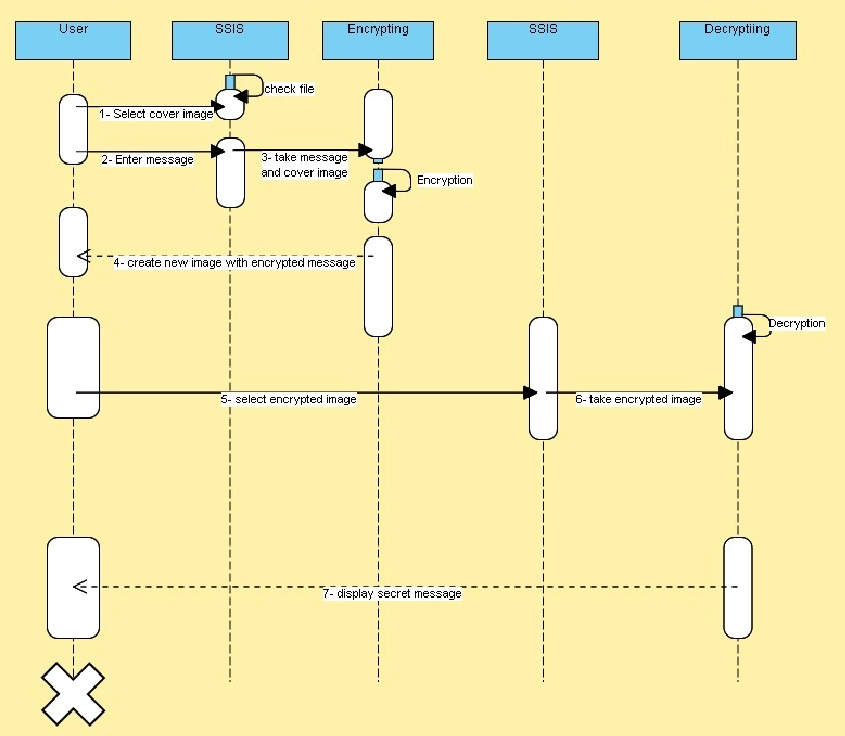
\includegraphics[width=35em, height=160mm]{figures/UML Design/Sequence Diagram.png}}
\caption{SSIS Sequence Diagram.}
\end{figure}
\vskip10em
\section{Activity diagram}
\vskip2em
\begin{figure}[ht!]
\centering
\frame{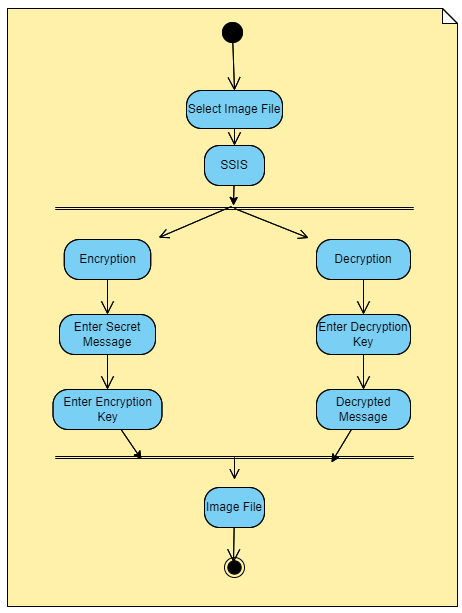
\includegraphics[width=35em, height=160mm]{figures/UML Design/Activity Diagram.png}}
\caption{SSIS Activity Diagram.}
\end{figure}
\vskip8em
\section{Class diagram}
\vskip2em
\begin{figure}[ht!]
\centering
\frame{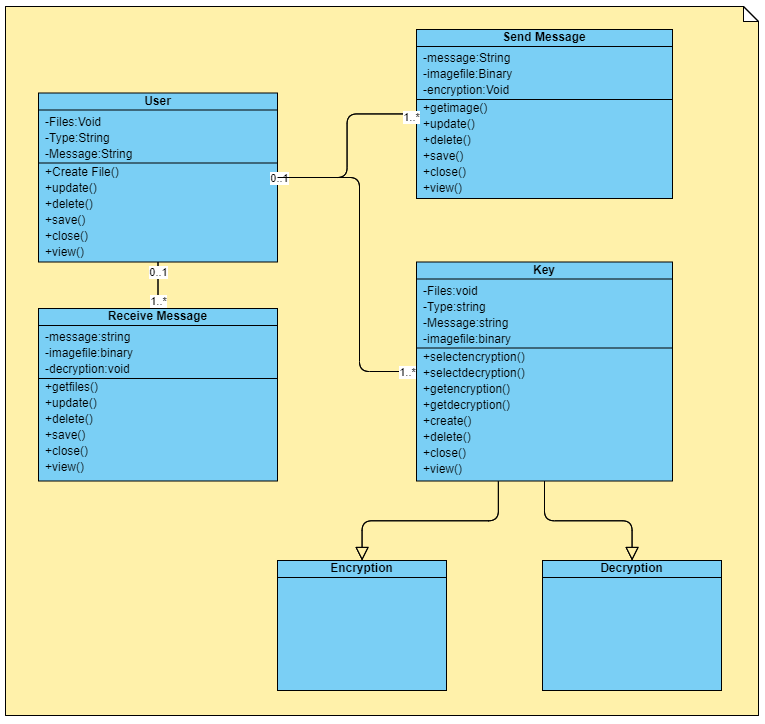
\includegraphics[width=35em, height=160mm]{figures/UML Design/Class Diagram.png}}
\caption{SSIS Class Diagram.}
\end{figure}


\chapter{SSIS Requirements Analysis}
\section{Functional requirements}
\subsection{Cover image selection and processing}
The SSIS system should allow the user to choose a suitable cover image, process it to ensure that it can be used for steganography, and ensure that it has enough area to embed the hidden message.
\subsection{Secret message encoding and encryption}
To ensure confidentiality, the system should encode the secret message in a way that it can be readily inserted into the cover image and then encrypt it using a safe algorithm.
\subsection{Embedding algorithm and SSIS application}
The SSIS system should have a strong embedding algorithm capable of inserting the encrypted message within the cover image without significantly modifying it.
\subsection{Extraction algorithm and SSIS application}
The system should have a trustworthy extraction algorithm capable of extracting the secret message from the stego-image.
\subsection{Decryption and decoding of the secret message}
The system should include a safe decryption algorithm capable of decrypting the encrypted message and revealing the original secret message.
\vskip6em
\section{Non-functional requirements}
\subsection{Performance}
The system should efficiently complete the embedding and extraction processes without generating substantial delays or compromising the quality of the cover image.
\vskip1em
\subsection{Security}
The system should ensure that unauthorised users cannot discover the embedded message and that the decrypted message stays confidential.
\vskip1em
\subsection{Scalability}
The system should be scalable and capable of handling a high volume of cover photos and texts.
\vskip1em
\subsection{User-friendliness}
The system should be simple to operate and come with detailed instructions.

\section{Key Takeaways}
\textbf{In conclusion, The SSIS system should provide a dependable and secure means of inserting hidden messages into cover images while maintaining confidentiality and authenticity.}

\chapter{SSIS High-Level Design}
\section{Architecture overview}
The SSIS system consists of five main components: Cover image selection and processing, Secret message encoding and encryption, Embedding algorithm and SSIS application, Extraction algorithm and SSIS application, and Decryption and decoding of the secret message.
\section{Cover image selection and processing}
The Cover Image Selection and Processing component of the SSIS system is responsible for selecting an appropriate cover image and processing it to ensure that it is suitable for embedding the secret message. The component may involve selecting an image with specific characteristics such as high resolution, minimal texture, or specific color combinations that can be used for steganography.

For example, in the SSIS system, the cover image may be selected based on the resolution and aspect ratio of the image. The image may be processed to ensure that it has enough space to embed the secret message and is in a suitable format for steganography.
\vskip6em
\section{Secret message encoding and encryption}
The SSIS system's Secret Message Encoding and Encryption component is in charge of encoding the secret message so that it may be easily incorporated into the cover image and encrypting it with a safe algorithm to assure confidentiality.

In the SSIS system, for example, the secret message might be encoded using a binary code that can easily be integrated into the cover image without materially affecting the image. To maintain confidentiality, the message can then be encrypted using a secure technique such as AES.

\section{Embedding algorithm}
The SSIS system's Embedding technique and SSIS Application component is in charge of embedding the encrypted message into the cover image using a robust technique. The component must ensure that the message is integrated in such a way that unauthorised users cannot discover it and that it does not significantly affect the cover image.

In the SSIS system, for example, the message may be embedded using a Least Significant Bit (LSB) technique, which substitutes the least significant bits of the cover picture pixels with the encrypted message bits. The SSIS application may also have extra features such as the ability to choose the embedding rate, which controls how much data can be buried in the image.

\section{Extraction algorithm}
The fourth SSIS system component is in charge of extracting the secret message from the stego-image. It employs a dependable extraction technique to find and extract the encoded message from the cover image while preserving the quality of the cover image.

To allow users to quickly extract messages from stego-images, the SSIS programme must provide a user-friendly interface. The user can choose a stego-image and begin the extraction process, and the application will provide feedback on the extraction's progress.

\section{Decryption and decoding of the secret message}
The SSIS system's last component is in charge of decrypting and decoding the secret message derived from the stego-image. It decrypts the encrypted message using a secure decryption technique to get the original secret message.
The SSIS programme must have an easy-to-use interface that allows users to simply decrypt and decode the secret message. The user can commence the decryption and decoding process by selecting an encrypted message, and the programme will provide feedback on the operation's progress.

\section{Key takeaways}
\textbf{The SSIS system architecture is flexible and scalable, ensuring quick secret message embedding and extraction. Its five components ensure confidentiality and authenticity by embedding hidden messages into cover images in a safe and secure manner. The system's components work in tandem to provide users with an easy-to-use and efficient solution for secret message communication. The system satisfies both functional and non-functional requirements, including performance, security, scalability, and usability.}


\chapter{Exchanged Messages and Data}
\section{Input data}
The input data in the SSIS system consists of a cover image and a secret message that the user wishes to place into the cover image. The cover image should be in a steganography-compatible format, and the secret message should be in text or any other supported format that may be encoded and encrypted.

Assume that the user wants to send a confidential message to a buddy via SSIS. They select a cover image, such as a sunset photograph, then type their message in a text file. The picture of the sunset and the text file containing the secret message would be the input data for SSIS.

\section{Output data}
The SSIS system's output data comprises of a stego-image and the decrypted message. The stego-image is the cover image that contains the secret message, and the decrypted message is the original secret message that the user intended to convey.

In our example, after the user enters the cover image and secret message into SSIS, the system will generate a stego-image, which is the same picture of the sunset but with the secret message contained inside it. When the friend receives the stego-image, they can utilise SSIS to extract and decode the secret message, resulting in the original message the user intended to send.
\vskip4em
\section{Message/data flow between components}
To enable the secure embedding, extraction, and decryption of the secret message, the SSIS system follows a precise message/data flow between its components.

First, the cover image is chosen and processed to guarantee it is steganographically suitable. The secret message is then encrypted and encoded using a safe technique. The encrypted message is subsequently embedded within the cover image by the SSIS system using a robust embedding method, resulting in the stego-image.

The stego-image is then put through the extraction algorithm, which extracts the secret message without modifying the cover image. Finally, the encrypted message is decoded using a secure decryption technique to yield the decrypted message.
\vskip4em
\section{Key takeaways}
\textbf{The SSIS system protects the security and confidentiality of data and messages exchanged between its components. The system can effectively embed, extract, and decode the secret message while retaining the integrity of the cover image by following the message/data flow between components.}

\chapter{Implementation details}
\vskip3em
\section{Programming language and libraries used}
\vskip2em
Any programming language with image processing and encryption libraries can be used to construct the SSIS system. Python, Java, and C++ are some of the most often used languages for building steganography systems.

Python is an appropriate language for SSIS since it offers a significant variety of libraries for image processing and encryption, such as OpenCV and cryptography. OpenCV is a popular image-processing toolkit that can be used for cover image selection, processing, and stego-image synthesis. Cryptography is a library that includes symmetric and asymmetric encryption methods that can be used for secret message encoding and encryption.

Pillow, a fork of the Python Imaging Library (PIL) that may be used for image processing and manipulation, and Stegano, a Python library for steganography that includes multiple embedding and extraction techniques, are two other libraries that can be used to build SSIS.
\vskip12em
\section{Sample code snippets}
\vskip1em
\begin{figure}[ht!]
\centering
\frame{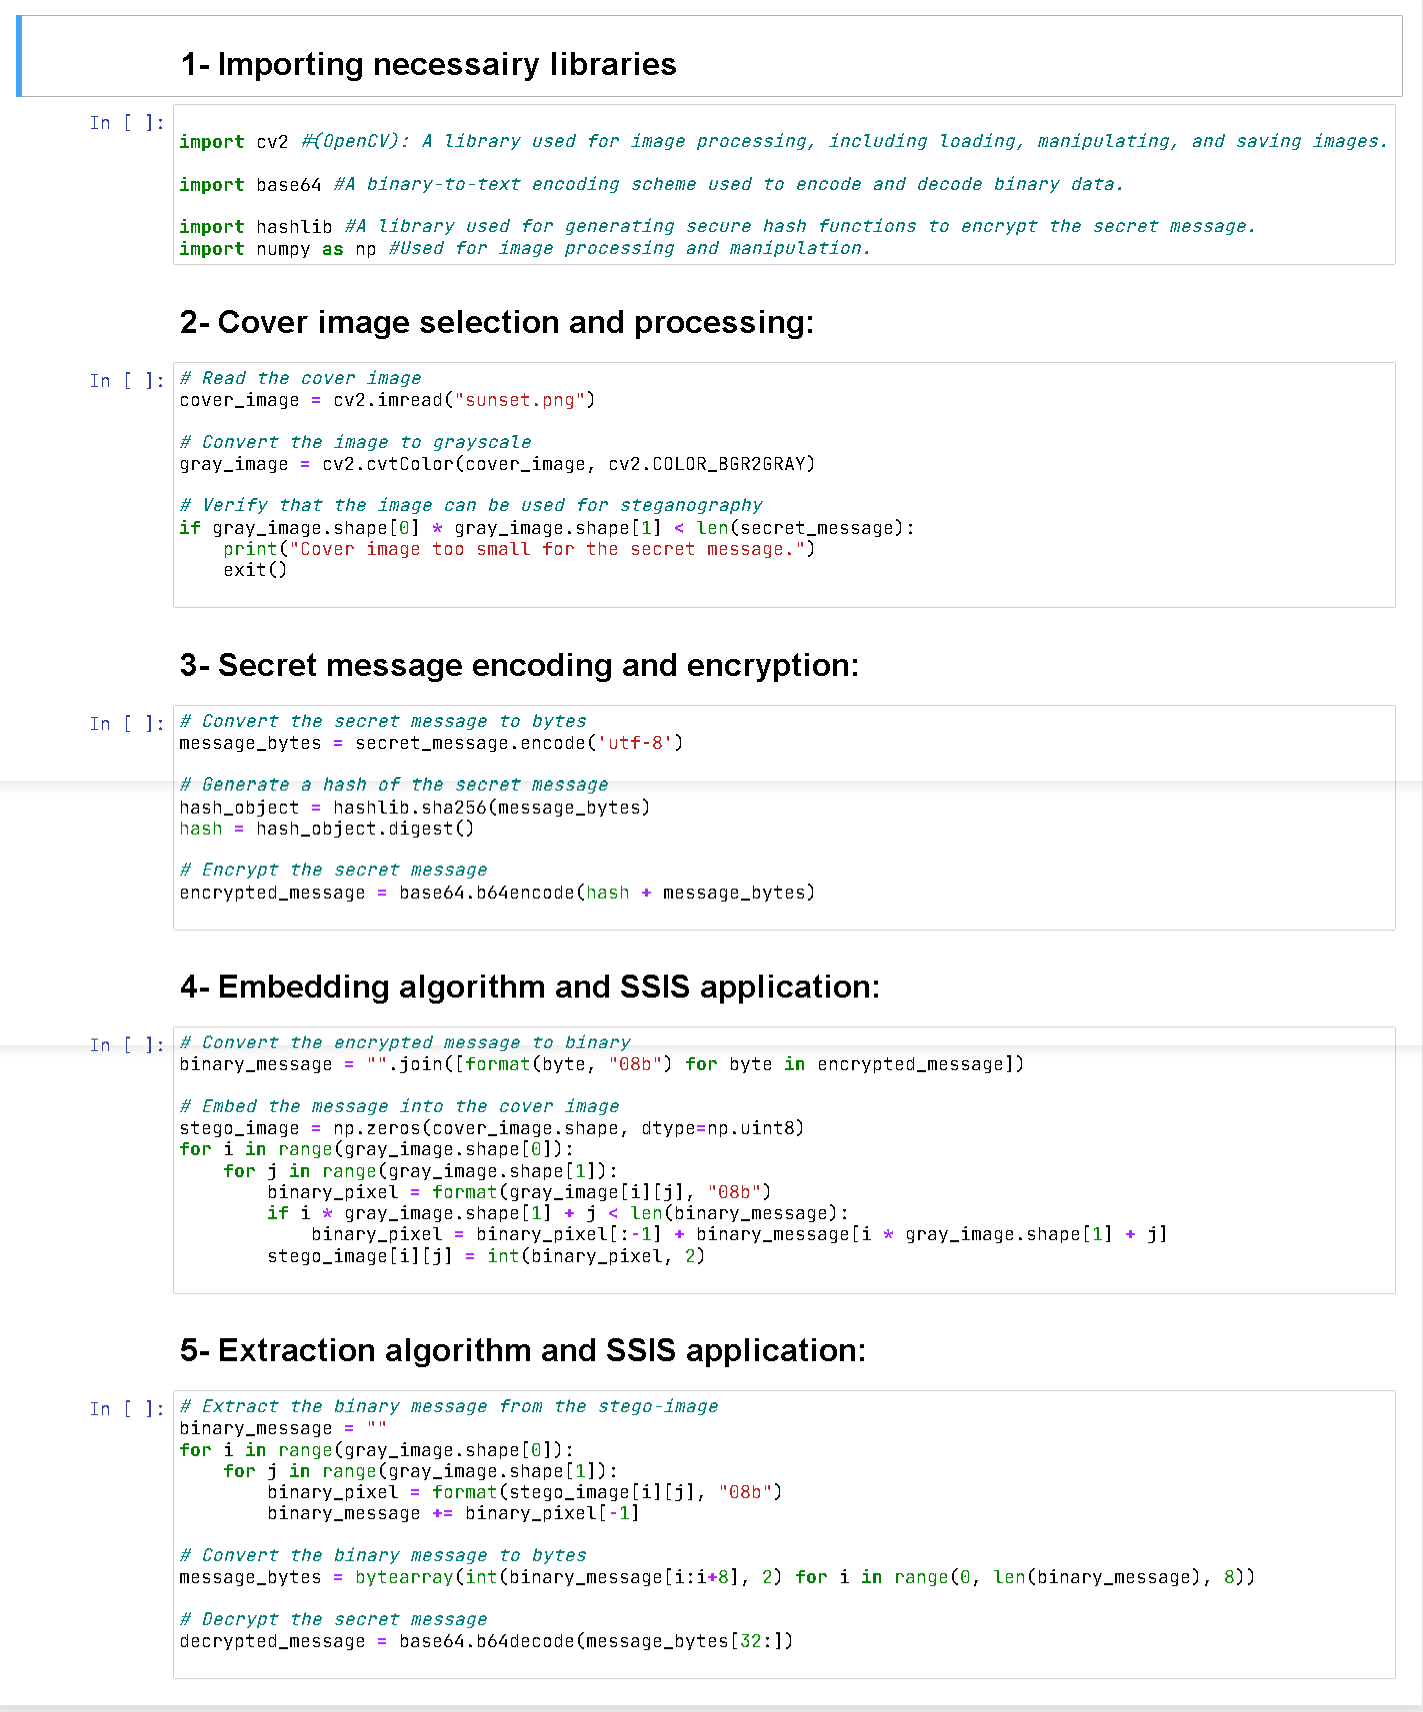
\includegraphics[width=37em, height=210mm]{figures/UML Design/Code snippet.png}}
\caption{SSID Python code snippet.}
\end{figure}

\section{Limitations and challenges}
The size of the secret message that can be placed in the cover image is restricted by the size of the cover image, which is one constraint of SSIS. Furthermore, if the cover image is compressed or altered, the encoded message may become corrupted or lost. Another issue is keeping the encoded message hidden from unauthorised users, as even minor alterations to the stego-image can reveal it.
\vskip3em
\section{Key Takeaways}
\textbf{SSIS can be implemented using a variety of programming languages and libraries, and it consists of numerous processes, including cover picture selection and processing, secret message encoding and encryption, embedding and extraction methods, and secret message decryption and decoding. When using SSIS, there are some restrictions and problems to consider.
SSIS offers a dependable and safe solution for inserting secret messages into cover images while maintaining secrecy and authenticity. The system is made up of multiple components that collaborate to pick and process the cover image, encode and encrypt the secret message, embed the message in the cover image, extract the message from the stego-image, and decrypt and decode the secret message.}
